\documentclass[12pt,a4paper, france]{article}

\newcommand{\workingDate}{\textsc{\selectlanguage{francais}\today}}
\newcommand{\userName}{DM 1}
\newcommand{\institution}{IODAA}
\newcommand\tab[1][1cm]{\hspace*{#1}}

\usepackage{researchdiary_png}


\begin{document}

\begin{center}
{\textbf {\huge DM1 : IA SOLVE}}\\[5mm]
{\large Auguste Gardette} \\[5mm]
{\text{ 20 Octobre 2022}} \\ [5mm]
\end{center}

\section{Recherche d’un chemin optimal par l’algorithme A${^*}$}

Soit le graphe correspondant \`a la figure 1 dans lequel les nombres sur les arcs indiquent le co${\hat{u}}$t
associ\'e \`a cet arc, et les nombres donn\'es pour chaque nœud indiquent la valeur retourn\'e par l\textquoteright heuristique pour ce nœud et le but « G ». \\


\begin{center}
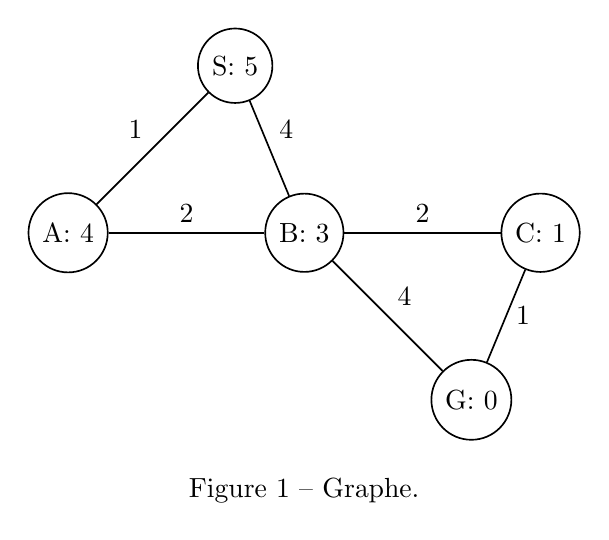
\begin{tikzpicture}[auto, node distance=3cm,semithick, main/.style = {draw, circle}]
\node[main] (1) {A: 4}; 
\node[main] (2) [right of=1] {B: 3}; 
\node[main] (3) [right of=2] {C: 1}; 
\node[main] (4) [above right of=1] {S: 5}; 
\node[main] (5) [below right of=2] {G: 0}; 
\node[below = 10] at (current bounding box.south) {Figure 1 – Graphe.};
\path [-]  (1) edge node {2} (2);
\path [-]  (2) edge node {2} (3);
\path [-]  (1) edge node {1} (4);
\path [-]  (4) edge node {4} (2);
\path [-]  (2) edge node {4} (5);
\path [-]  (5) edge node[right] {1} (3);
\end{tikzpicture} \\ [5mm]
\end{center}


Donnez l\textquoteright ordre d\textquoteright exploration des nœuds d\'evelopp\'es par une recherche en meilleur d\textquoteright abord commençant par le nœud  « S ». Montrez l\textquoteright \'evolution des listes OUVERT et FERM\'E. \\

\begin{tabular}{ | c || *{2}{c|}}
    \hline
    Tour & Ouvert & Ferm\'e  \\
    \hline
    \hline
    0 & S(0 + 5) & \\
    \hline
    1 & A(1 + 4); B(4 + 3) & S(5)\\
    \hline
    2 & B(3 + 3) par A; B(7) par S & S(5); A(5)\\
    \hline
    3 & C(5 + 1); G(7 + 0) & S(5); A(5); B(6) par A \\
    \hline
    4 & G(6 + 0) par C G(7) par B & S(5); A(5); B(6) par A; C(6)\\
    \hline
    4 & & S(5); A(5); B(6) par A; C(6); G(6) par C\\
    \hline
\end{tabular} \\

Le Chemin optimal retourn\'e par l\textquoteright algorithme du meilleur d\textquoteright abord est : \\
\tab \tab \tab S ${\rightarrow}$ A ${\rightarrow}$ B ${\rightarrow}$ C ${\rightarrow}$ G\\

\section{Optimalit\'e de l\textquoteright algorithme A${^*}$}

Prouvez que l\textquoteright algorithme A${^*}$ retourne un chemin de co${\hat{u}}$t optimal si la fonction heuristique h(n) est admissible. \\

Supposons un chemin optimal C${^*}$ mais que notre algorithme retourne C > C${^*}$. Quelque soit C, on est n\'ecessairement pass\'e par un nœud optimal. \\

On aurait donc : \tab \tab  \;  \;  \; f(n) ${>}$ C${^*}$ \\
\tab Par d\'efinition : \tab \tab \tab f(n) = g(n) + h(n) \\
\tab n sur le chemin optimal : \tab \, f(n) = g${^*}$(n) + h(n) \\
\tab h(n) admissible :  \tab \tab \; \; \, f(n) ${\le}$ g${^*}$(n) + h${^*}$(n) \\
\tab Contradiction : \tab \tab \tab f(n) ${\le}$ C${^*}$(n) \\

Donc si f(n) est plus faible en co${\hat{u}}$t que f${^*}$(n), f${^*}$(n) ne sera jamais explor\'e car non-optimal. h(n) admissible retourne donc n\'ecessairement le chemin optimal.

\section{Transformation de A${^*}$ pour trouver un chemin le plus long}

L\textquoteright algorithme A${^*}$  permet de trouver un plus court chemin dans un graphe. On va chercher ici
comment le transformer pour qu\textquoteright il permette de trouver un plus long chemin. \\

1. Que se passe-t-il si on n\textquoteright utilise pas de fonction heuristique ? \\

Si on n\textquoteright utilise pas de fonction heuristique, on a un risque de ne trouver aucun chemin jusqu\textquoteright au nœud objectif et de boucler infiniement.\\ 

\tab 2. Quelle doit ${\hat{e}}$tre la propri\'et\'e d\textquoteright une fonction heuristique pour que le chemin retourn\'e soit un plus long chemin ? \\

La fonction heuristique doit n\'ecessairemet  ${\hat{e}}$tre admissible pour trouver un chemin valide. \\

\tab 3. Donner l\textquoteright algorithme retournant un plus long chemin. \\

Pour chaque tour, on choisit dans notre liste ouverte le nœud n donc la fonction f(n) est la plus co${\hat{u}}$teuse et dont il existe au moins un nœuds voisins pouvant encore ${\hat{e}}$tre d\'evelopp\'es jusqu\textquoteright \`a atteindre l\textquoteright objectif. \\

\tab 4. Le tester sur le petit graphe de la figure 1 et montrer l\textquoteright ordre d\textquoteright exploration des nœuds. \\

\begin{tabular}{ | c || *{2}{c|}}
    \hline
    Tour & Ouvert & Ferm\'e  \\
    \hline
    \hline
    0 & S(0 + 5) & \\
    \hline
    1 & A(1 + 4); B(4 + 3) & S(5)\\
    \hline
    2 & G(8 + 0); C(6 + 1); A(1 + 4) par S; A(6 + 4) par B *& S(5); B(7)\\
    \hline
    3 & & A(5); B(7); G(8) \\
    \hline
\end{tabular} \\
* Au tour 2, le nœud A n\textquoteright est pas admissible par il n\textquoteright y a pas de noeud pouvant ${\hat{e}}$tre d\'evelopp\'e apr\`es et que ce n\textquoteright est pas un noeud objectif.\\

Le Chemin retourn\'e par l\textquoteright algorithme du plus long d\textquoteright abord est : \\
\tab \tab \tab S ${\rightarrow}$ B ${\rightarrow}$ G\\


\section{Jeu \`a trois joueurs}

Comment pourrait-on modifier l\textquoteright algorithme minimax pour qu\textquoteright il soit utilisable dans le cas d\textquoteright un jeu \`a information parfaite \`a trois joueurs ? \\
Par exemple, consid\'erons un jeu \`a trois joueurs nomm\'es 0, 1 et 2 (voir figure 2). On va supposer que la fonction d\textquoteright \'evaluation retourne un triplet de valeurs indiquant l\textquoteright \'evaluation de la position pour les joueurs 0, 1 et 2. Par exemple, le triplet (6, 2, 4) indique que cette position est tr\`es d\'esirable pour le joueur 0, nettement moins pour le joueur 1 et moyennement pour le joueur 2.\\

1. Compl\'eter l’arbre de jeu de la figure 2 en remplissant les triplets jusqu\textquoteright \`a la racine.\\

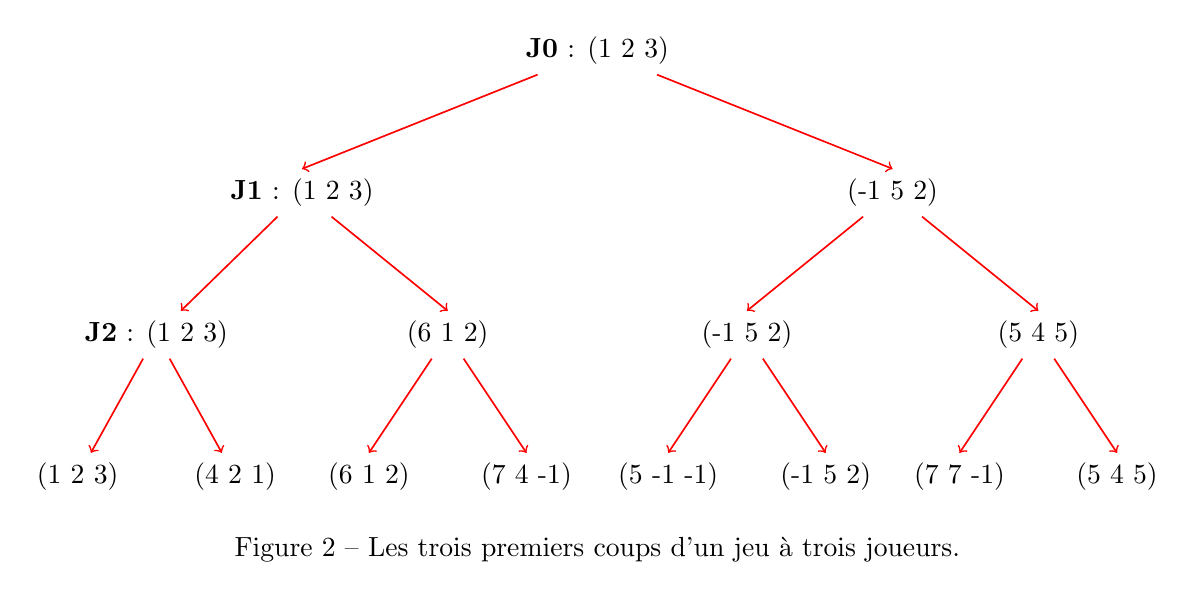
\begin{tikzpicture}[auto, node distance=3.4cm,semithick, level 1/.style={sibling distance=7.5cm},
level 2/.style={sibling distance=3.7cm}, level 3/.style={sibling distance=2cm}, level 4/.style={sibling distance=1.3cm}]
\node (1) {\textbf{J0} : (1 2 3)}
    child{[draw=red, ->] node [below] {\textbf{J1} : (1 2 3)}
        child{  node [below] {\textbf{J2} : (1 2 3)}
            child{ node [below] {(1 2 3)} 
            } 
            child{ node [below] {(4 2 1)}
            }
        }
        child{[->] node [below] {(6 1 2)}
            child{ [->] node [below] {(6 1 2)}
            }
            child{[->] node [below] {(7 4 -1)}
            }
        }
    }
    child{[draw=red, ->] node [below] {(-1 5 2)}
        child{[->] node [below] {(-1 5 2)}
            child{ [->] node [below] {(5 -1 -1)}
            }
            child{[->] node [below] {(-1 5 2)}
            }
        }
        child{[->] node [below] {(5 4 5)}
            child{ [->] node [below] {(7 7 -1)}
            }
            child{[->] node [below] {(5 4 5)}
            }
        }
    };
\node[below = 10] at (current bounding box.south) {Figure 2 – Les trois premiers coups d\textquoteright un jeu \`a trois joueurs.};
\end{tikzpicture} \\ [5mm]

2. R\'e-\'ecrire le programme MinMax pour qu\textquoteright il joue correctement sur ce type d\textquoteright arbre. \\

Algorithmes de remont\'ee des \'etiquettes num\'eriques : \\
\tab \tab - Si J0 : Max des valeurs pour la position 0 dans les triplets des successeurs.\\
\tab \tab - Si J1 : Max des valeurs pour la position 1 dans les triplets des successeurs.\\
\tab \tab - Si J2 : Max des valeurs pour la position 2 dans les triplets des successeurs.\\

G\'en\'eralisation du programme MinMax pour ce type de jeu : \\
- Soit n joueurs : Si Ji : Max des valeurs pour la position i dans les n-uplets des successeurs.\\

Dans le cas o\`u les valeurs \`a la position i dans les n-uplets des succeurs pour un joueur i sont identiques, on pourrait rajouter dans notre algortihme la r\`egle suvante : \\
- Ji cherche \`a minimiser la somme total du gain de ses adversaires dans le cas d\textquoteright une \'egalit\'es des valeurs \`a la position i du n-uplet. \\

Mais l\textquoteright objectif d\textquoteright un jeu ne doit pas n\'ecessairement de faire perdre le plus possible ses adversaires... surtout s\textquoteright il y a plusieur parties (apr\`es on risque de rentrer dans une notion de dilemme du prisionnier).

\end{document}